\chapter{Réalisation}	

	\section{Installation et configuration de l'application}
	
	Notre projet est codé en Python 3. Des fichiers XML sont utilisés pour le stockage des vaisseaux. Pour la partie système expert il nécessaire d'avoir un shell (par exemple cygwin sur Windows) pour que le programme puisse appeler des commandes UNIX externes comme \textit{make}.


	\section{Organisation et répartition des tâches}

	Au premier semestre, nous avions dégagé 4 domaines de travail : le programme du moteur de combat, la construction d'une base de données issues du jeu original, les tests et enfin le rapport.\\
Le moteur de combat a été réalisé en partie par Simon BIHEL avec la contribution de Julien PEZANT pour la classe des armes et l'aide de Sébastien GAMBLIN pour une partie de l'affichage.\\
La construction de la base de données a été faite en collaboration par Julien PEZANT, Paul LEMENAGER et Simon BIHEL.\\
Les tests ont été faits en partie par Josselin GUENERON, Sébastien GAMBLIN et en partie par Simon BIHEL.\\
Enfin le rapport a été construit par Simon BIHEL et Sébastien GAMBLIN avec la contribution de chacun des autres membres par rapport à leurs connaissances du projet.

	Au second semestre, nous avons dégagé 4 domaines de travail : l'enrichissement et l'amélioration du moteur de combats ; l'optimisation et la recherche des meilleurs vaisseaux ; des affichages divers pour les vaisseaux et les tournois ; la rédaction du rapport. \\
La travail sur le moteur de combats et sur la recherche des meilleurs vaisseaux a été effectué par Simon BIHEL. \\
Les affichages ont été réalisés par Sébastien GAMBLIN. \\
Le rapport a été dirigé par Simon BIHEL avec l'apport de chacun des membres. Notamment, Julien PEZANT a participé à la refonte et traduction des schémas du rapport du premier semestre et Sébastien GAMBLIN a rédigé la partie des affichages.
		

	\section{Importation des modules}
	
	\begin{figure}[H]
		\caption{Diagramme des packages}
		\label{fig:packages}
		\centering
		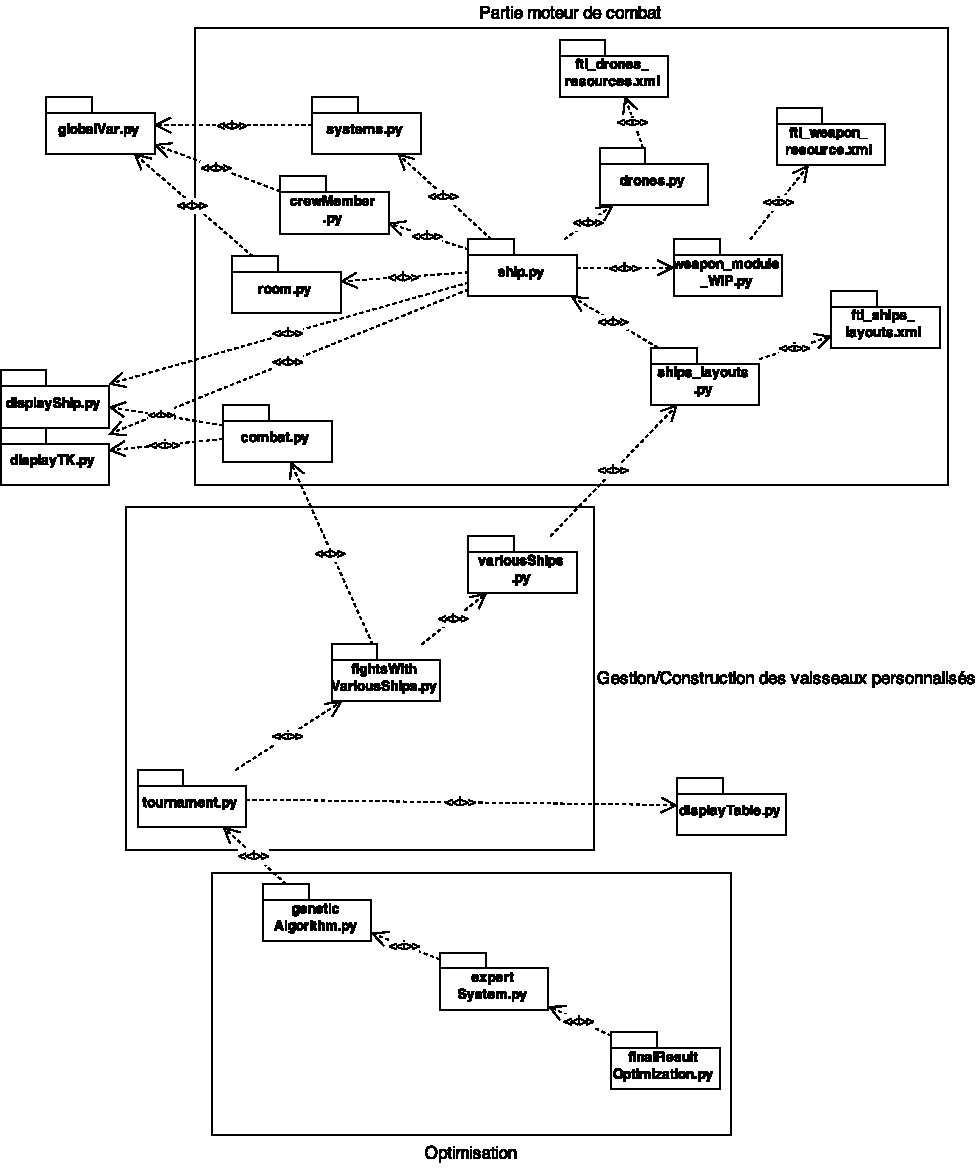
\includegraphics[width=1.2\linewidth]{packageDiagram.pdf}
	\end{figure}
	
	Comme on peut le voir dans la figure~\ref{fig:packages}, notre programme est divisé en 3 grandes parties :
	\begin{itemize}
		\item une partie qui gère les combats entre vaisseaux (réalisé au semestre 1) ;
		\item une partie qui gère les vaisseaux personnalisés ;
		\item une partie qui utilise les 2 parties précédentes pour déterminer le meilleur vaisseau.
	\end{itemize}
	En plus de cela, il y a aussi diverses fonctions d'affichage (graphiques ou textuelles) ainsi qu'un fichier qui contient des variables globales qui déterminent s'il doit y avoir certains affichages, la division du temps pour le moteur de combats, etc.

	
	\section{Détermination de divers paramètres}
	
	Dans les algorithmes utilisés il a certaines variables arbitraires qui permettent de faire des tests ou encore de faire un certain nombre de boucles. Pour déterminer au mieux ces variables il a fallu avoir certaines réflexions et effectuer certaines expérimentations.

	\paragraph{Les tournois} Dans un tournoi, les vaisseaux font des matchs entre eux et le gagnant d'un match est celui qui aura gagné plus de combats que son adversaire. Pour être assuré que ce soit presque toujours le meilleur vaisseau qui gagne le match il a fallu trouver un bon nombre de combats pour avoir des résultats corrects et un temps raisonnable pour le tournoi complet. À noter aussi que nous avons choisi un nombre impair pour éviter des matchs nuls (sachant qu'un combat a toujours un gagnant). Nous avons choisi 21.

	\paragraph{Les algorithmes génétiques} Ici, le paramètre qui peut rendre un algorithme génétique obsolète est le nombre maximal de générations. Celui-ci est là pour éviter qu'un \textit{metagame} s'installe et empêche l'algorithme de finir. Un \textit{metagame} est une mode dans les stratégies de jeu. La limite de générations doit donc donner assez de temps aux vaisseaux de se perfectionner sans gaspiller du temps sur des changements de mode. Nous avons choisi d'avoir 30 générations. Ensuite, il y a la stabilisation qui dépend du ratio de victoires maximal pour déterminer si un vaisseau est plus fort que les autres ou si tous les vaisseaux sont à peu près équivalents en terme de nombre de victoires. Nous avons choisi de dire qu'un vaisseau est plus fort que les autres s'il gagne plus des deux tiers de ses matchs.

	\paragraph{L'algorithme final} Plusieurs paramètres ont dû être déterminés dans l'algorithme final de recherche du meilleur vaisseau.\\
Le taux de confiance minimum pour le taux de croissance est de \sfrac{1}{3} car cela veut dire que le taux de croissance est d'au plus \sfrac{1}{2}. C'est-à-dire que si 1\% des bons vaisseaux ont une caractéristique, alors au maximum 2\% des mauvais l'auront. Étant donné la grande différence entre le nombre de mauvais vaisseaux et de bons, on aura les caractéristiques vraiment propres aux bons vaisseaux, cependant il faut avoir bon équilibre dans la proportion du nombre de champions retenus dans une population au cours d'un algorithme génétique. Une taille de population 5 fois supérieure au nombre de champions d'une génération semble marcher au final (pas de réelle réflexion scientifique ici, juste une constatation).\\
Le nombre d'algorithmes génétiques au début doit être plus grand que 1 pour ne pas avoir un seul modèle de vaisseau et donc le meilleur vaisseau au final sera identique ou très proche du vainqueur de l'algorithme génétique. Il n'y a pas de maximum car cela enrichira simplement la diversité des vaisseaux et permettra d'essayer plus de bonnes combinaisons d'équipement. À noter que ce sont les algorithmes génétiques qui prennent la majorité du temps, et le temps croît de façon exponentielle en fonction du nombre de combats par match, du nombre de vaisseaux dans une population, etc.
	
	\section{Divers résultats d'optimisation}
	
	La visualisation de données peut être un exercice compliqué mais nous pouvons regarder l'évolution de l'équipement des vaisseaux au cours d'un algorithme d'optimisation.
	
	Regardons un exemple d'algorithme génétique avec stabilisation avec une population de 20 individus et 2 champions et un coût de 600 scraps. La population de base est composée (aléatoirement) d'engi cruisers de tous types. Une première étape peut être de faire construire une base de données pour chaque génération avec le programme de data mining LCM. Rappelons les caractéristiques principales de chaque type d'engi cruiser. Le type A a l'arme Ion Blast II et le drone Combat I. Le type B a les armes Heavy Ion et Heavy Laser I. Le type C a l'arme Dual Laser et le drone Beam I.
	
	Pour la population de base, étant donnée la construction aléatoire des vaisseaux, les équipements communs sont ceux de base comme l'énergie, le système des armes ou les boucliers. Les champions sont deux engi cruisers C, l'engi0 et l'engi1. Ces deux vaisseaux ont les augmentations suivantes. L'engi0 a 3 d'énergie, 5 dans le système des armes, 1 dans les moteurs, 2 dans le système des drones, les armes antibioBeam et glaiveBeam et le drone beam1. L'engi1 a 2 d'énergie, 6 dans les boucliers, 1 dans l'invisibilité, 1 dans les moteurs et le drone combat1.
	
	La seconde génération est composée des deux champions précédents et de vaisseaux issus du croisement des deux champions, deux de ces nouveaux vaisseaux ont subi une mutation. En plus des équipements communs de la première génération, on voit que trois quarts des vaisseaux ont l'antiobioBeam. Les champions sont toujours l'engi0 et l'engi1.
	
	Après plusieurs générations on arrive à la dernière, l'engi0 et l'engi1 sont toujours les champions. Parmi les derniers vaisseaux, l'antibioBeam est toujours dans les trois quarts des vaisseaux.
	
	Au final, les croisements n'ont pas créé de meilleurs vaisseaux, sans doute car les équipements des deux champions n'étaient pas compatibles et les mutations n'ont pas réussi non plus à créer de bons vaisseaux.
	
	
	\section{Failles et inexactitude des résultats}

	Notre programme présente quelques failles et n'est pas complet par rapport au jeu originel ce qui rend les résultats donnés pas forcément applicables dans de vraies parties. Voici quelques points à prendre en compte pour la validité des résultats donnés par le programme.
	
	
	\paragraph{Le moteur de combats} Tous les équipements du jeu ne sont pas gérés par le moteur de combats. À cause de cela, les vaisseaux issus des algorithmes de génération et d'optimisation n'auront pas certains équipements qui sont potentiellement bons. De plus, L'Intelligence Artificielle qui dirige les vaisseaux fait les choses bêtement et n'utilise pas forcément des techniques de jeu. Cela peut rendre des vaisseaux obsolètes alors qu'ils sont bons quand ils sont bien utilisés.

	\paragraph{La génération aléatoire de vaisseaux} Le fait de pouvoir vendre de l'équipement n'est pas présent dans le générateur aléatoire, donc ce n'est pas présent dans les algorithmes d'optimisation. À cause de cela, il a encore beaucoup de vaisseaux potentiellement bons qui ne sont pas utilisés.

	\paragraph{L'algorithme génétique} L'algorithme génétique peut s'enfermer dans un \textit{matchup}. C'est-à-dire qu'il peut créer des vaisseaux performants dans un seul type de combat et mauvais contre la plupart des vaisseaux qui ne sont pas présents dans la population de cet algorithme génétique. Au fil du temps et malgré le nombre maximal de générations, un \textit{metagame} peut s'installer et dans ce cas il est difficile de différencier une évolution utile d'un effet de mode.
	
	\paragraph{L'algorithme final} Dans l'algorithme final, la base de vaisseaux est constituée à partir d'algorithmes génétiques, donc les champions auront certaines caractéristiques en commun avec les mauvais, cela peut faire baisser le taux de croissance et le taux de confiance. Cela est amplifié par le fait que les algorithmes génétiques s'arrêtent par stabilisation car dans certains cas, les individus de la dernière génération seront similaires. 
